\documentclass[12pt,letterpaper]{article}
\usepackage[utf8]{inputenc}
\usepackage{tikz}
\usepackage[hidelinks]{hyperref}
\author{Curso de \LaTeX}
\title{Figuras geométricas con TikZ}
\begin{document}
\maketitle

Aunque podemos dibujar cualquier figura en 2D con las opciones vistas antes, existen instrucciones especiales para dibujar algunas figuras geométricas más fácilmente.

\section*{Rectángulos}

Por ejemplo, para dibujar un rectángulo:

\begin{tikzpicture}
\draw (0,0) rectangle (2,3);
\end{tikzpicture}

Si queremos dibujar figuras geométricas con relleno, cambiamos el comando \textbackslash\texttt{draw} por \textbackslash\texttt{fill}:


\begin{tikzpicture}
	\fill[orange] (0,0) rectangle (2,3);
\end{tikzpicture}

Este comando requiere definir un color de relleno para la figura dibujada, de otra forma no es visible. El comando \textbackslash\texttt{shade} tiene un comportamiento similar:


\begin{tikzpicture}
\shade[top color=yellow, bottom color=black] (0,0) rectangle (1,2);
\end{tikzpicture}

Con el añadido de que la figura cuenta con un color de relleno degradado. Las opciones ``\texttt{top color=}'' y ``\texttt{bottom color=}'' sirven para indicar la dirección de la degradación y los colores involucrados. 

Finalmente \textbackslash\texttt{filldraw} permite combinar las características de los comandos \textbackslash\texttt{draw} y \textbackslash\texttt{fill}, obteniendo una figura con contorno y relleno:


\begin{tikzpicture}
\filldraw[fill=green!20!white, draw=green!40!black] (0,0) rectangle (2,1);
\end{tikzpicture}

Las opciones \texttt{fill} y \texttt{draw} se utilizan para indicar el color del relleno y el borde de la figura, respectivamente. El color de relleno ``green!20!white'' significa 20\% verde y 80\% blanco mezclados juntos.

\section*{Círculos y elipses}

Los cículos y las elipses se dibujan iniciando indicando su centro, entonces utilizamos la instrucción ``circle'' para dibujar su circunferencia. Este comando debe estar acompañado de una opción que indique el tamaño de su radio o de dos opciones que indiquen las longitudes de los semiejes de la elipse:

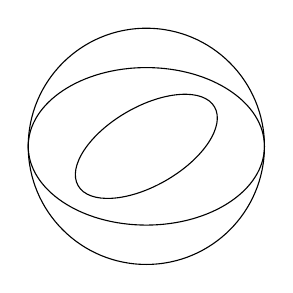
\begin{tikzpicture}
\draw (0,0) circle [radius=1.5];
\draw (0,0) circle [x radius=1.5cm, y radius=10mm];
\draw (0,0) circle [x radius=1cm, y radius=5mm, rotate=30];
\end{tikzpicture}

\section*{Arcos}

La instrucción ``arc'' crea una parte de un círculo o una elipse:

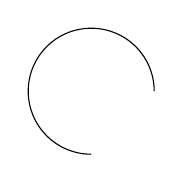
\begin{tikzpicture}
\draw (0,0) arc (0:270:8mm);
\end{tikzpicture}

\begin{tikzpicture}
\draw (0,0) arc (25:325:1.75cm and 1cm);
\end{tikzpicture}

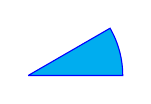
\begin{tikzpicture}
\filldraw[fill=cyan, draw=blue] (0,0) -- (12mm,0mm) arc (0:30:12mm) -- (0,0);
\end{tikzpicture}



\section*{Cuadrículas}

Podemos dibujar cuadriculas empleando la instrucción ``grid'':

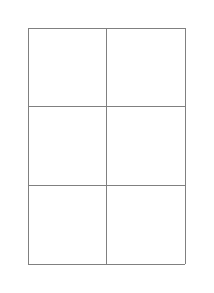
\begin{tikzpicture}
\draw[help lines] (0,0) grid (2,3); % La opción <helps lines> denota ``gris fino''
\end{tikzpicture}

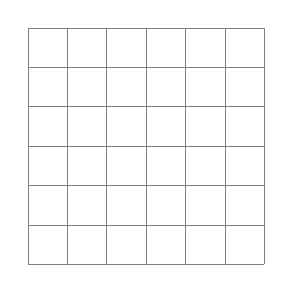
\begin{tikzpicture}
\draw[step=0.5, gray, very thin] (-1.5,-1.5) grid (1.5,1.5);
\end{tikzpicture}

Estas cuadriculas pueden ser muy útiles para ayudarnos a ubicar la posición de los elementos dentro del plano, por ejemplo, si combinamos ``grid'' con ``arc'', podemos visualizar el punto desde donde se origina el arco y como lo afectan los parámetros de su instrucción:

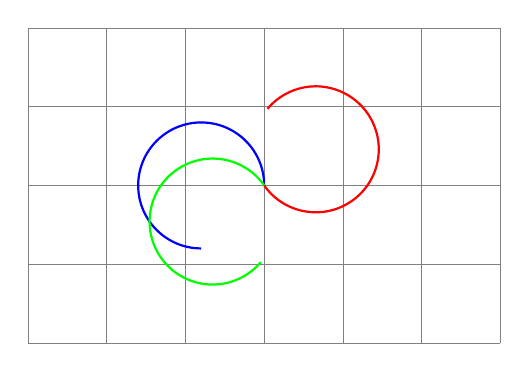
\begin{tikzpicture}
\draw[help lines] (-3,-2) grid (3,2); 
\draw[thick, blue] (0,0) arc (0:270:8mm);
\draw[thick, green] (0,0) arc (35:320:8mm);
\draw[thick, red] (0,0) arc (35:320:-8mm);
\end{tikzpicture}


\section*{Parábolas, senos y cosenos}

Hay varias instrucciones para dibujar curvas especiales que describan funciones matemáticas, como ``parabola'', ``sin'', ``cos'' (curso de seno o coseno en el intervalo $ [0,\pi/2] $).

Para dibujar parábolas:

\begin{tikzpicture}
\draw (0,0) parabola (1,1.5) parabola[bend at end] (2,0);
\end{tikzpicture}

Para dibujar curvas de seno y coseno:

\begin{tikzpicture}
\draw (0,0) sin (1,1) cos (2,0) sin (3,-1) cos (4,0) sin (5,1);
\end{tikzpicture}

\section*{Agregar flechas a los dibujos}

Para añadir flechas existen una opción muy sencilla:

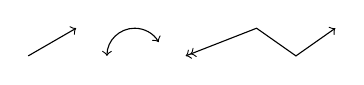
\begin{tikzpicture}
\draw [->] (0,0) -- (30:20pt); 
\draw [<->] (1,0) arc (180:30:10pt); 
\draw [<<->] (2,0) -- ++(0.9,10pt) -- ++(0.5,-10pt) -- ++(0.5,10pt);
\end{tikzpicture}

\end{document}